\documentclass{article}
\usepackage{spconf,amsmath,graphicx,booktabs,multirow,microtype,url,balance}
% ===== macros printed by main.tex. Each value is emitted by a script from a JSON receipt; see the emitters in relabel_v1/ and scenes_v1/. Re-run relabel_v1/tidy_numbers.py after any emitter. =====
\newcommand{\AdjFramePairs}{2,280}
\newcommand{\ChainBoxes}{4,336}
\newcommand{\ChainFramePairsReg}{1,748}
\newcommand{\DupDiffType}{44}
\newcommand{\DupFrames}{51}
\newcommand{\DupPairs}{53}
\newcommand{\EmDownBeer}{15.9}
\newcommand{\EmDownHigh}{11.9}
\newcommand{\EmDownWater}{18.5}
\newcommand{\EmDownWine}{11.0}
\newcommand{\EmUpBeer}{0.9}
\newcommand{\EmUpShot}{8.9}
\newcommand{\EmUpWater}{4.7}
\newcommand{\EmUpWine}{0.8}
\newcommand{\FlipCountReg}{502}
\newcommand{\FlipNeighbourPct}{87}
\newcommand{\FlipPairsReg}{2,775}
\newcommand{\FlipRateReg}{18.1}
\newcommand{\ImagesTrainScene}{1,750}
\newcommand{\ManOODFlipRate}{0.3}
\newcommand{\ManOODFlips}{1}
\newcommand{\ManOODPairs}{316}
\newcommand{\ManStdFlipRate}{0.0}
\newcommand{\ManStdFlips}{0}
\newcommand{\ManStdPairs}{93}
\newcommand{\ManualChainOOD}{0 of 351}
\newcommand{\ManualChainStd}{0 of 167}
\newcommand{\ManualGeThreeOOD}{346 of 351}
\newcommand{\ManualGeThreeStd}{163 of 167}
\newcommand{\ManualMedianOOD}{15}
\newcommand{\ManualMedianStd}{10}
\newcommand{\PairSShotOODMax}{+52.6}
\newcommand{\PairSShotOODMean}{+8.2}
\newcommand{\PairSShotOODMedian}{+1.8}
\newcommand{\PairSShotOODPos}{3/5}
\newcommand{\PairSShotStdMean}{$-$4.1}
\newcommand{\PairSWaterOODMean}{+8.0}
\newcommand{\PairSWaterOODPos}{4/5}
\newcommand{\PairSWaterStdMean}{+3.2}
\newcommand{\PairSWhiskyOODMean}{+14.9}
\newcommand{\PairSWhiskyOODPos}{4/5}
\newcommand{\PairSWhiskyStdMean}{$-$6.9}
\newcommand{\PairSWineOODMean}{+11.1}
\newcommand{\PairSWineOODPos}{4/5}
\newcommand{\PairSWineStdMean}{+3.8}
\newcommand{\RatioManualOOD}{1.83}
\newcommand{\RatioManualStd}{0.79}
\newcommand{\RatioRawTrain}{0.58}
\newcommand{\RatioSceneTrain}{0.51}
\newcommand{\SceneBoxesGeThree}{3,953}
\newcommand{\SceneBoxesGeThreePct}{91}
\newcommand{\SceneChains}{786}
\newcommand{\SceneChanged}{535}
\newcommand{\SceneChangedPct}{12.3}
\newcommand{\SceneEpochs}{300}
\newcommand{\SceneHops}{2}
\newcommand{\SceneMedianLen}{10}
\newcommand{\SceneRefused}{64}
\newcommand{\SceneRegPairs}{4,097}
\newcommand{\SceneRepeatSlots}{1,538}
\newcommand{\SceneSlots}{3,288}
\newcommand{\SceneTied}{140}
\newcommand{\SceneTol}{0.5}
\newcommand{\SceneTriedPairs}{4,465}
\newcommand{\SceneUpdates}{15,600}
\newcommand{\ScenesHeld}{25}
\newcommand{\ScenesTrain}{70}
\newcommand{\SelRsq}{0.04}
\newcommand{\SvCells}{5}
\newcommand{\SvGenStdVsRawGain}{$-$1.7}
\newcommand{\SvLCells}{5}
\newcommand{\SvLRecOODVsRawGainL}{$-$1.7}
\newcommand{\SvLRecOODVsRawPosL}{2}
\newcommand{\SvLRecStdVsRawGainL}{+0.5}
\newcommand{\SvLRecStdVsRawPosL}{2}
\newcommand{\SvLSixOODVsRawGainL}{+11.1}
\newcommand{\SvLSixStdVsRawGainL}{$-$1.7}
\newcommand{\SvLTypeOODVsRawGainL}{+11.3}
\newcommand{\SvLTypeOODVsRawPosL}{5}
\newcommand{\SvLTypeStdVsRawGainL}{$-$0.6}
\newcommand{\SvLTypeStdVsRawPosL}{2}
\newcommand{\SvOODAbove}{3}
\newcommand{\SvOODBelow}{1}
\newcommand{\SvOODStraddle}{1}
\newcommand{\SvRecStdVsRawCI}{[$-$3.7, $-$0.3]}
\newcommand{\SvSixOODTrkVsRawGain}{+0.7}
\newcommand{\SvSixOODVsRawCI}{[+1.8, +12.3]}
\newcommand{\SvSixOODVsRawGain}{+7.1}
\newcommand{\SvSixOODVsRawPos}{5}
\newcommand{\SvSixOODVsTrkCI}{[+0.6, +12.2]}
\newcommand{\SvSixOODVsTrkGain}{+6.4}
\newcommand{\SvSixStdVsRawGain}{$-$1.9}
\newcommand{\SvStdAbove}{1}
\newcommand{\SvStdBelow}{1}
\newcommand{\SvTypeOODTrkVsRawGain}{+5.0}
\newcommand{\SvTypeOODVsRawCI}{[$-$5.7, +24.1]}
\newcommand{\SvTypeOODVsRawGain}{+9.2}
\newcommand{\SvTypeOODVsRawPos}{4}
\newcommand{\SvTypeOODVsRawSD}{12.0}
\newcommand{\SvTypeOODVsTrkGain}{+4.0}
\newcommand{\SvTypeOODVsTrkPos}{4}
\newcommand{\SvTypeStdVsRawGain}{+0.8}
\newcommand{\SvTypeStdVsTrkGain}{$-$1.8}
\newcommand{\TrkChains}{1,561}
\newcommand{\TrkChanged}{364}
\newcommand{\TrkChangedPct}{8.4}
\newcommand{\TrkMedianVotes}{5.5}
\newcommand{\TrkSingletons}{878}
\newcommand{\WhiskyShareOOD}{11.7}
\newcommand{\WhiskyShareRaw}{25.9}
\newcommand{\WhiskyShareStd}{17.4}
\newcommand{\XHostTypeOOD}{14.3}
\newcommand{\XHostTypeStd}{10.9}

% SUPERSEDED. Nothing below is used by main.tex. Kept for provenance of earlier drafts only; recompute before citing any of it.
\newcommand{\AdjBot}{58.2}
\newcommand{\AdjScenes}{91}
\newcommand{\AdjTop}{57.6}
\newcommand{\ApsrEpochs}{300}
\newcommand{\ApsrUpdates}{21,000}
\newcommand{\BaseEpochs}{553}
\newcommand{\BaseSeedOneStdSix}{77.16}
\newcommand{\BaseTwentyOneOODGen}{3.01}
\newcommand{\BaseTwentyOneOODSix}{$-$0.62}
\newcommand{\BaseTwentyOneStdGen}{1.27}
\newcommand{\BaseTwentyOneStdSix}{3.40}
\newcommand{\BaseUpdates}{21,014}
\newcommand{\BootCells}{6}
\newcommand{\BootImgPos}{4}
\newcommand{\BootLoMax}{7.28}
\newcommand{\BootLoMin}{1.09}
\newcommand{\BootPreExcl}{1}
\newcommand{\BootPreOODList}{[$-$9.3, +1.1], [+5.3, +17.0], [$-$1.9, +6.7]}
\newcommand{\BootPreStdList}{[$-$8.6, +0.0], [$-$0.7, +13.0], [$-$10.7, +1.4]}
\newcommand{\BootRtxOODHi}{+13.9}
\newcommand{\BootRtxOODLo}{+6.1}
\newcommand{\BootRtxStdHi}{+13.5}
\newcommand{\BootRtxStdLo}{+0.0}
\newcommand{\BoxMaxDiff}{$5\times10^{-7}$}
\newcommand{\BudgetOnlyGen}{1.98}
\newcommand{\BudgetOnlySix}{5.49}
\newcommand{\ChainMedianLen}{1}
\newcommand{\ChainTracks}{1,561}
\newcommand{\ChalkOODGenMean}{1.23}
\newcommand{\ChalkOODSixA}{0.90}
\newcommand{\ChalkOODSixB}{11.60}
\newcommand{\ChalkOODSixC}{6.97}
\newcommand{\ChalkOODSixMax}{11.60}
\newcommand{\ChalkOODSixMean}{6.49}
\newcommand{\ChalkOODSixMin}{0.90}
\newcommand{\ChalkSceneMax}{16.84}
\newcommand{\ChalkSceneMin}{2.12}
\newcommand{\ChalkStdGenMean}{0.51}
\newcommand{\ChalkStdSixA}{6.80}
\newcommand{\ChalkStdSixB}{6.55}
\newcommand{\ChalkStdSixC}{4.79}
\newcommand{\ChalkStdSixMax}{6.80}
\newcommand{\ChalkStdSixMean}{6.05}
\newcommand{\ChalkStdSixMin}{4.79}
\newcommand{\CoatAllCells}{18}
\newcommand{\CoatAllMean}{2.47}
\newcommand{\CoatAllPositive}{15}
\newcommand{\CoatOtherMean}{0.57}
\newcommand{\CoatRosterBMean}{0.73}
\newcommand{\CoatRosterCMean}{0.40}
\newcommand{\CoatRosterCount}{3}
\newcommand{\CoatRosterEMean}{6.27}
\newcommand{\ComparisonCount}{6}
\newcommand{\DispBot}{14.59}
\newcommand{\DispMax}{29.98}
\newcommand{\DispMin}{0.045}
\newcommand{\DispTop}{1.25}
\newcommand{\DrawOODGen}{0.26}
\newcommand{\DrawOODSix}{1.23}
\newcommand{\DrawStdGen}{2.14}
\newcommand{\DrawStdSix}{3.51}
\newcommand{\EligCells}{6}
\newcommand{\EligMax}{13.32}
\newcommand{\EligMean}{7.84}
\newcommand{\EligMin}{3.81}
\newcommand{\EligPositive}{6}
\newcommand{\EmDownShot}{0.0}
\newcommand{\EmDownWhisky}{9.4}
\newcommand{\EmHighDown}{11.9}
\newcommand{\EmShotUp}{8.9}
\newcommand{\EmUpHigh}{0.0}
\newcommand{\EmUpWhisky}{3.1}
\newcommand{\EmWhiskyDown}{9.4}
\newcommand{\EpochRatio}{1.84}
\newcommand{\FlipBeerWineReg}{51}
\newcommand{\FlipBeerWineUnreg}{23}
\newcommand{\FlipCountUnreg}{183}
\newcommand{\FlipOtherMaxReg}{5}
\newcommand{\FlipOtherMaxUnreg}{5}
\newcommand{\FlipPairsUnreg}{902}
\newcommand{\FlipRateUnreg}{20.3}
\newcommand{\FlipRegPairList}{shot/whisky 137, whisky/water 117, water/beer 89, beer/wine 51, wine/high 42, whisky/beer 22, water/wine 16, shot/water 11}
\newcommand{\FlipShotWaterReg}{11}
\newcommand{\FlipShotWhiskyReg}{137}
\newcommand{\FlipShotWhiskyUnreg}{24}
\newcommand{\FlipWaterBeerReg}{89}
\newcommand{\FlipWaterBeerUnreg}{40}
\newcommand{\FlipWaterWineReg}{16}
\newcommand{\FlipWhiskyBeerReg}{22}
\newcommand{\FlipWhiskyWaterReg}{117}
\newcommand{\FlipWhiskyWaterUnreg}{42}
\newcommand{\FlipWineHighReg}{42}
\newcommand{\FlipWineHighUnreg}{29}
\newcommand{\GenSelMaxAbs}{3.27}
\newcommand{\GenericMaxAbs}{2.79}
\newcommand{\GradedBootCells}{6}
\newcommand{\GradedBootWrong}{3}
\newcommand{\GradedCells}{4}
\newcommand{\GradedMarginFour}{1.47}
\newcommand{\GradedMarginTwo}{$-$2.26}
\newcommand{\GradedRuns}{18}
\newcommand{\GridBMean}{0.73}
\newcommand{\GridCMean}{0.40}
\newcommand{\GridGeoMean}{7.84}
\newcommand{\GridMean}{2.99}
\newcommand{\GridPositive}{15}
\newcommand{\GridTotal}{18}
\newcommand{\HeldBoxes}{1,065}
\newcommand{\HeldIdsChangedPct}{10.0}
\newcommand{\HoldScenes}{25}
\newcommand{\HoldWinsA}{7}
\newcommand{\HoldWinsB}{18}
\newcommand{\HoldWinsC}{15}
\newcommand{\ImagesHeld}{625}
\newcommand{\MsdGenOODGain}{+1.2}
\newcommand{\MsdGenOODRawHMean}{66.1}
\newcommand{\MsdGenOODRawHSD}{0.88}
\newcommand{\MsdGenOODRawRMean}{67.4}
\newcommand{\MsdGenOODRawRSD}{1.07}
\newcommand{\MsdGenOODRelHMean}{67.3}
\newcommand{\MsdGenOODRelHSD}{0.99}
\newcommand{\MsdGenOODRelRMean}{66.9}
\newcommand{\MsdGenOODRelRSD}{2.06}
\newcommand{\MsdGenStdGain}{+0.8}
\newcommand{\MsdGenStdRawHMean}{84.0}
\newcommand{\MsdGenStdRawHSD}{2.22}
\newcommand{\MsdGenStdRawRMean}{84.4}
\newcommand{\MsdGenStdRawRSD}{1.56}
\newcommand{\MsdGenStdRelHMean}{84.8}
\newcommand{\MsdGenStdRelHSD}{2.98}
\newcommand{\MsdGenStdRelRMean}{87.2}
\newcommand{\MsdGenStdRelRSD}{0.51}
\newcommand{\MsdRecOODGain}{+3.1}
\newcommand{\MsdRecOODRawHMean}{77.9}
\newcommand{\MsdRecOODRawHSD}{4.05}
\newcommand{\MsdRecOODRawRMean}{82.3}
\newcommand{\MsdRecOODRawRSD}{1.42}
\newcommand{\MsdRecOODRelHMean}{81.0}
\newcommand{\MsdRecOODRelHSD}{0.82}
\newcommand{\MsdRecOODRelRMean}{78.8}
\newcommand{\MsdRecOODRelRSD}{1.00}
\newcommand{\MsdRecStdGain}{$-$1.0}
\newcommand{\MsdRecStdRawHMean}{89.6}
\newcommand{\MsdRecStdRawHSD}{1.25}
\newcommand{\MsdRecStdRawRMean}{92.5}
\newcommand{\MsdRecStdRawRSD}{0.90}
\newcommand{\MsdRecStdRelHMean}{88.6}
\newcommand{\MsdRecStdRelHSD}{1.20}
\newcommand{\MsdRecStdRelRMean}{89.5}
\newcommand{\MsdRecStdRelRSD}{2.69}
\newcommand{\MsdSeedsH}{3}
\newcommand{\MsdSeedsR}{2}
\newcommand{\MsdSixOODGain}{+0.3}
\newcommand{\MsdSixOODRawHMean}{53.8}
\newcommand{\MsdSixOODRawHSD}{7.09}
\newcommand{\MsdSixOODRawRMean}{53.5}
\newcommand{\MsdSixOODRawRSD}{0.32}
\newcommand{\MsdSixOODRelHMean}{54.0}
\newcommand{\MsdSixOODRelHSD}{4.56}
\newcommand{\MsdSixOODRelRMean}{54.8}
\newcommand{\MsdSixOODRelRSD}{5.23}
\newcommand{\MsdSixStdGain}{$-$4.3}
\newcommand{\MsdSixStdRawHMean}{68.9}
\newcommand{\MsdSixStdRawHSD}{3.91}
\newcommand{\MsdSixStdRawRMean}{60.1}
\newcommand{\MsdSixStdRawRSD}{1.13}
\newcommand{\MsdSixStdRelHMean}{64.6}
\newcommand{\MsdSixStdRelHSD}{4.63}
\newcommand{\MsdSixStdRelRMean}{67.0}
\newcommand{\MsdSixStdRelRSD}{1.96}
\newcommand{\MsdTypeOODGain}{+3.0}
\newcommand{\MsdTypeOODRawHMean}{77.9}
\newcommand{\MsdTypeOODRawHSD}{7.28}
\newcommand{\MsdTypeOODRawRMean}{67.9}
\newcommand{\MsdTypeOODRawRSD}{3.40}
\newcommand{\MsdTypeOODRelHMean}{80.9}
\newcommand{\MsdTypeOODRelHSD}{0.38}
\newcommand{\MsdTypeOODRelRMean}{75.9}
\newcommand{\MsdTypeOODRelRSD}{5.32}
\newcommand{\MsdTypeStdGain}{$-$0.7}
\newcommand{\MsdTypeStdRawHMean}{86.1}
\newcommand{\MsdTypeStdRawHSD}{4.15}
\newcommand{\MsdTypeStdRawRMean}{76.2}
\newcommand{\MsdTypeStdRawRSD}{0.19}
\newcommand{\MsdTypeStdRelHMean}{85.4}
\newcommand{\MsdTypeStdRelHSD}{2.76}
\newcommand{\MsdTypeStdRelRMean}{83.3}
\newcommand{\MsdTypeStdRelRSD}{0.68}
\newcommand{\PairCandidates}{2,129}
\newcommand{\PairSOODNegCount}{0}
\newcommand{\PairSShotStdMax}{+10.4}
\newcommand{\PairSShotStdMedian}{$-$9.8}
\newcommand{\PairSShotStdPos}{1/5}
\newcommand{\PairSStdNegCount}{2}
\newcommand{\PairSWaterOODMax}{+23.6}
\newcommand{\PairSWaterOODMedian}{+11.8}
\newcommand{\PairSWaterStdMax}{+19.3}
\newcommand{\PairSWaterStdMedian}{$-$1.6}
\newcommand{\PairSWaterStdPos}{2/5}
\newcommand{\PairSWhiskyOODMax}{+41.3}
\newcommand{\PairSWhiskyOODMedian}{+15.2}
\newcommand{\PairSWhiskyStdMax}{+14.5}
\newcommand{\PairSWhiskyStdMedian}{$-$12.7}
\newcommand{\PairSWhiskyStdPos}{1/5}
\newcommand{\PairSWineOODMax}{+28.2}
\newcommand{\PairSWineOODMedian}{+11.3}
\newcommand{\PairSWineStdMax}{+13.9}
\newcommand{\PairSWineStdMedian}{+2.6}
\newcommand{\PairSWineStdPos}{4/5}
\newcommand{\PairSelected}{2,068}
\newcommand{\PairShotWhiskyOODMean}{-7.2}
\newcommand{\PairShotWhiskyOODPos}{1}
\newcommand{\PairShotWhiskyStdMean}{-1.4}
\newcommand{\PairShotWhiskyStdPos}{0}
\newcommand{\PairVOODNegCount}{2}
\newcommand{\PairVShotOODMax}{+23.6}
\newcommand{\PairVShotOODMean}{$-$2.4}
\newcommand{\PairVShotOODMedian}{$-$12.7}
\newcommand{\PairVShotOODPos}{2/5}
\newcommand{\PairVShotStdMax}{+4.1}
\newcommand{\PairVShotStdMean}{$-$1.7}
\newcommand{\PairVShotStdMedian}{$-$2.0}
\newcommand{\PairVShotStdPos}{1/5}
\newcommand{\PairVStdNegCount}{1}
\newcommand{\PairVWaterOODMax}{+36.8}
\newcommand{\PairVWaterOODMean}{+15.8}
\newcommand{\PairVWaterOODMedian}{+13.7}
\newcommand{\PairVWaterOODPos}{4/5}
\newcommand{\PairVWaterStdMax}{+25.8}
\newcommand{\PairVWaterStdMean}{+6.9}
\newcommand{\PairVWaterStdMedian}{+6.7}
\newcommand{\PairVWaterStdPos}{3/5}
\newcommand{\PairVWhiskyOODMax}{+13.7}
\newcommand{\PairVWhiskyOODMean}{+1.8}
\newcommand{\PairVWhiskyOODMedian}{+0.0}
\newcommand{\PairVWhiskyOODPos}{2/5}
\newcommand{\PairVWhiskyStdMax}{+17.9}
\newcommand{\PairVWhiskyStdMean}{+1.9}
\newcommand{\PairVWhiskyStdMedian}{$-$1.9}
\newcommand{\PairVWhiskyStdPos}{2/5}
\newcommand{\PairVWineOODMax}{+4.5}
\newcommand{\PairVWineOODMean}{$-$3.9}
\newcommand{\PairVWineOODMedian}{+0.0}
\newcommand{\PairVWineOODPos}{2/5}
\newcommand{\PairVWineStdMax}{+14.3}
\newcommand{\PairVWineStdMean}{+1.0}
\newcommand{\PairVWineStdMedian}{+2.6}
\newcommand{\PairVWineStdPos}{3/5}
\newcommand{\PairWaterBeerOODMean}{+13.6}
\newcommand{\PairWaterBeerOODPos}{2}
\newcommand{\PairWaterBeerStdMean}{+0.7}
\newcommand{\PairWaterBeerStdPos}{1}
\newcommand{\PairWhiskyWaterOODMean}{+4.2}
\newcommand{\PairWhiskyWaterOODPos}{2}
\newcommand{\PairWhiskyWaterStdMean}{-5.6}
\newcommand{\PairWhiskyWaterStdPos}{0}
\newcommand{\PairWineHighOODMean}{-3.6}
\newcommand{\PairWineHighOODPos}{1}
\newcommand{\PairWineHighStdMean}{-1.5}
\newcommand{\PairWineHighStdPos}{2}
\newcommand{\PoolCells}{5}
\newcommand{\PoolExclList}{H200 seed 3407 OOD [+5.3, +17.0], RTX seed 1337 OOD [+6.1, +13.9], RTX seed 5678 standard [+2.0, +13.7] and RTX seed 5678 OOD [+1.4, +10.4]}
\newcommand{\PoolGenOODGain}{+0.5}
\newcommand{\PoolGenOODPos}{3}
\newcommand{\PoolGenStdGain}{+1.6}
\newcommand{\PoolGenStdPos}{3}
\newcommand{\PoolRecOODGain}{+0.5}
\newcommand{\PoolRecOODPos}{3}
\newcommand{\PoolRecStdGain}{$-$1.8}
\newcommand{\PoolRecStdPos}{1}
\newcommand{\PoolSixOODGain}{+0.7}
\newcommand{\PoolSixOODPos}{2}
\newcommand{\PoolSixStdGain}{+0.2}
\newcommand{\PoolSixStdPos}{3}
\newcommand{\PoolTypeCases}{10}
\newcommand{\PoolTypeExclNeg}{0}
\newcommand{\PoolTypeExclZero}{4}
\newcommand{\PoolTypeOODGain}{+5.0}
\newcommand{\PoolTypeOODPos}{4}
\newcommand{\PoolTypeStdGain}{+2.4}
\newcommand{\PoolTypeStdPos}{3}
\newcommand{\PreregHashA}{5f5014b294ee9c69202f2c42d841d82d}
\newcommand{\PreregHashB}{6bf583aabe5ce3f664846be2cb4b7645}
\newcommand{\ProbeCells}{12}
\newcommand{\ProbePositive}{9}
\newcommand{\RatioManualTest}{1.40}
\newcommand{\RatioRelTrain}{0.54}
\newcommand{\RelCells}{6}
\newcommand{\RelLabelsHashA}{18479ef702f3ce3dc887ec04014f3d85}
\newcommand{\RelLabelsHashB}{99b85b5d4aa8bc41524f6f53647529f3}
\newcommand{\RelLastCellsAll}{5}
\newcommand{\RelLastRecOODGain}{0.28}
\newcommand{\RelLastRecOODPos}{1}
\newcommand{\RelLastRecStdGain}{-3.79}
\newcommand{\RelLastRecStdPos}{0}
\newcommand{\RelLastSixOODGain}{6.72}
\newcommand{\RelLastSixOODPos}{3}
\newcommand{\RelLastSixOODPosAll}{5}
\newcommand{\RelLastSixStdGain}{-2.56}
\newcommand{\RelLastSixStdPos}{0}
\newcommand{\RelLastSixStdPosAll}{0}
\newcommand{\RelLastTypeOODGain}{6.01}
\newcommand{\RelLastTypeOODPos}{3}
\newcommand{\RelLastTypeOODPosAll}{4}
\newcommand{\RelLastTypeSdOODRaw}{5.99}
\newcommand{\RelLastTypeSdOODRel}{3.11}
\newcommand{\RelLastTypeSdStdRaw}{1.56}
\newcommand{\RelLastTypeSdStdRel}{2.82}
\newcommand{\RelLastTypeStdGain}{0.05}
\newcommand{\RelLastTypeStdPos}{2}
\newcommand{\RelLastTypeStdPosAll}{2}
\newcommand{\RelPreregHashA}{9e810aefb279e29efcd84242b947d792}
\newcommand{\RelPreregHashB}{a37239fd7b324359a798699245bb1908}
\newcommand{\RelRecLessPos}{5}
\newcommand{\RelRecOODGain}{3.13}
\newcommand{\RelRecOODPos}{3}
\newcommand{\RelRecStdGain}{-1.00}
\newcommand{\RelRecStdPos}{0}
\newcommand{\RelSceneWinsOOD}{0/3, 2/3, 2/3}
\newcommand{\RelSceneWinsStd}{0/3, 2/3, 0/3}
\newcommand{\RelSixOODGain}{0.26}
\newcommand{\RelSixOODPos}{1}
\newcommand{\RelSixPosAll}{2}
\newcommand{\RelSixStdGain}{-4.28}
\newcommand{\RelSixStdPos}{1}
\newcommand{\RelTypeOODGain}{2.99}
\newcommand{\RelTypeOODPos}{2}
\newcommand{\RelTypePosAll}{3}
\newcommand{\RelTypeSdOODRaw}{7.28}
\newcommand{\RelTypeSdOODRel}{0.38}
\newcommand{\RelTypeSdStdRaw}{4.15}
\newcommand{\RelTypeSdStdRel}{2.76}
\newcommand{\RelTypeStdGain}{-0.72}
\newcommand{\RelTypeStdPos}{1}
\newcommand{\RelabelDirections}{shot$\to$whisky 61, whisky$\to$water 49, water$\to$beer 36, whisky$\to$shot 30, water$\to$whisky 30, beer$\to$wine 25, beer$\to$water 24, wine$\to$high 23}
\newcommand{\RelabelledBoxes}{364}
\newcommand{\RelabelledPct}{8.4}
\newcommand{\RelabelledVal}{25}
\newcommand{\RepCleanRecOODGain}{0.76}
\newcommand{\RepCleanRecOODPos}{3}
\newcommand{\RepCleanRecStdGain}{-0.00}
\newcommand{\RepCleanRecStdPos}{1}
\newcommand{\RepCleanSixOODGain}{3.80}
\newcommand{\RepCleanSixOODPos}{2}
\newcommand{\RepCleanSixStdGain}{-0.69}
\newcommand{\RepCleanSixStdPos}{1}
\newcommand{\RepCleanTypeOODGain}{6.93}
\newcommand{\RepCleanTypeOODPos}{2}
\newcommand{\RepCleanTypeStdGain}{-0.02}
\newcommand{\RepCleanTypeStdPos}{1}
\newcommand{\RepOODSixA}{2.77}
\newcommand{\RepOODSixB}{9.46}
\newcommand{\RepOODSixC}{1.53}
\newcommand{\RepOODSixMean}{4.59}
\newcommand{\RepStdSixA}{$-$7.87}
\newcommand{\RepStdSixB}{0.30}
\newcommand{\RepStdSixC}{3.84}
\newcommand{\RepStdSixMean}{$-$1.24}
\newcommand{\RescoreCells}{6}
\newcommand{\RescoreDeltas}{+1.1, +1.0, +2.0, +0.9, $-$0.3, +2.2}
\newcommand{\RescorePos}{5}
\newcommand{\RosterBFailed}{59}
\newcommand{\RosterBOODSix}{11.04}
\newcommand{\RosterBStdSix}{$-$4.65}
\newcommand{\RosterCFailed}{60}
\newcommand{\RosterMinShared}{2,007}
\newcommand{\RosterShared}{2,008}
\newcommand{\RosterSwapped}{60}
\newcommand{\RosterSwappedPct}{1.35}
\newcommand{\SceneCount}{6}
\newcommand{\ScenePreregHashA}{4788e631014d366fb00cd8c81f55d9ba}
\newcommand{\ScenePreregHashB}{29ae4758a78afe32be12ff82ec5aa1c9}
\newcommand{\SceneValChanged}{30}
\newcommand{\SeedCount}{3}
\newcommand{\SelArbCount}{3}
\newcommand{\SelCells}{6}
\newcommand{\SelMax}{10.57}
\newcommand{\SelMean}{5.08}
\newcommand{\SelMin}{-2.94}
\newcommand{\SelOODMean}{6.87}
\newcommand{\SelPositive}{5}
\newcommand{\SelRunCount}{9}
\newcommand{\SelSdStd}{2.69}
\newcommand{\SelSdStdWorst}{6.87}
\newcommand{\SelStdMean}{3.29}
\newcommand{\SelectionRate}{97.13}
\newcommand{\ShareManualTest}{18.9\slash 13.5\slash 17.8\slash 21.6\slash 11.8\slash 16.4}
\newcommand{\ShareRawTrain}{15.0\slash 25.9\slash 17.0\slash 14.6\slash 16.7\slash 10.8}
\newcommand{\SlotCount}{4,443}
\newcommand{\SvExclCases}{10}
\newcommand{\SvExclNeg}{2}
\newcommand{\SvExclPos}{4}
\newcommand{\SvGenOODTrkVsRawGain}{+0.5}
\newcommand{\SvGenOODTrkVsRawPos}{3}
\newcommand{\SvGenOODVsRawCI}{[$-$3.0, +2.2]}
\newcommand{\SvGenOODVsRawGain}{$-$0.3}
\newcommand{\SvGenOODVsRawPos}{2}
\newcommand{\SvGenOODVsRawSD}{2.1}
\newcommand{\SvGenOODVsTrkCI}{[$-$3.1, +1.4]}
\newcommand{\SvGenOODVsTrkGain}{$-$0.9}
\newcommand{\SvGenOODVsTrkPos}{2}
\newcommand{\SvGenOODVsTrkSD}{1.8}
\newcommand{\SvGenStdTrkVsRawGain}{+1.6}
\newcommand{\SvGenStdTrkVsRawPos}{3}
\newcommand{\SvGenStdVsRawCI}{[$-$6.8, +3.4]}
\newcommand{\SvGenStdVsRawPos}{1}
\newcommand{\SvGenStdVsRawSD}{4.1}
\newcommand{\SvGenStdVsTrkCI}{[$-$6.8, +0.2]}
\newcommand{\SvGenStdVsTrkGain}{$-$3.3}
\newcommand{\SvGenStdVsTrkPos}{1}
\newcommand{\SvGenStdVsTrkSD}{2.8}
\newcommand{\SvLGenOODTrkVsRawGain}{+1.3}
\newcommand{\SvLGenOODTrkVsRawPos}{4}
\newcommand{\SvLGenOODVsRawGain}{+0.2}
\newcommand{\SvLGenOODVsRawGainL}{+0.2}
\newcommand{\SvLGenOODVsRawPos}{3}
\newcommand{\SvLGenOODVsRawPosL}{3}
\newcommand{\SvLGenOODVsTrkGain}{$-$1.1}
\newcommand{\SvLGenOODVsTrkPos}{0}
\newcommand{\SvLGenStdTrkVsRawGain}{+0.8}
\newcommand{\SvLGenStdTrkVsRawPos}{3}
\newcommand{\SvLGenStdVsRawGain}{+1.0}
\newcommand{\SvLGenStdVsRawGainL}{+1.0}
\newcommand{\SvLGenStdVsRawPos}{3}
\newcommand{\SvLGenStdVsRawPosL}{3}
\newcommand{\SvLGenStdVsTrkGain}{+0.2}
\newcommand{\SvLGenStdVsTrkPos}{2}
\newcommand{\SvLRecOODTrkVsRawGain}{+0.2}
\newcommand{\SvLRecOODTrkVsRawPos}{2}
\newcommand{\SvLRecOODVsRawGain}{$-$1.7}
\newcommand{\SvLRecOODVsRawPos}{2}
\newcommand{\SvLRecOODVsTrkGain}{$-$1.9}
\newcommand{\SvLRecOODVsTrkPos}{1}
\newcommand{\SvLRecStdTrkVsRawGain}{$-$2.3}
\newcommand{\SvLRecStdTrkVsRawPos}{1}
\newcommand{\SvLRecStdVsRawGain}{+0.5}
\newcommand{\SvLRecStdVsRawPos}{2}
\newcommand{\SvLRecStdVsTrkGain}{+2.8}
\newcommand{\SvLRecStdVsTrkPos}{3}
\newcommand{\SvLSixOODTrkVsRawGain}{+7.0}
\newcommand{\SvLSixOODTrkVsRawPos}{5}
\newcommand{\SvLSixOODVsRawGain}{+11.1}
\newcommand{\SvLSixOODVsRawPos}{5}
\newcommand{\SvLSixOODVsRawPosL}{5}
\newcommand{\SvLSixOODVsTrkGain}{+4.1}
\newcommand{\SvLSixOODVsTrkPos}{5}
\newcommand{\SvLSixStdTrkVsRawGain}{$-$4.4}
\newcommand{\SvLSixStdTrkVsRawPos}{0}
\newcommand{\SvLSixStdVsRawGain}{$-$1.7}
\newcommand{\SvLSixStdVsRawPos}{1}
\newcommand{\SvLSixStdVsRawPosL}{1}
\newcommand{\SvLSixStdVsTrkGain}{+2.7}
\newcommand{\SvLSixStdVsTrkPos}{5}
\newcommand{\SvLTypeOODTrkVsRawGain}{+6.9}
\newcommand{\SvLTypeOODTrkVsRawPos}{4}
\newcommand{\SvLTypeOODVsRawGain}{+11.3}
\newcommand{\SvLTypeOODVsRawPos}{5}
\newcommand{\SvLTypeOODVsTrkGain}{+3.4}
\newcommand{\SvLTypeOODVsTrkPos}{4}
\newcommand{\SvLTypeStdTrkVsRawGain}{$-$2.2}
\newcommand{\SvLTypeStdTrkVsRawPos}{2}
\newcommand{\SvLTypeStdVsRawGain}{$-$0.6}
\newcommand{\SvLTypeStdVsRawPos}{2}
\newcommand{\SvLTypeStdVsTrkGain}{+0.5}
\newcommand{\SvLTypeStdVsTrkPos}{2}
\newcommand{\SvRecOODTrkVsRawGain}{+0.5}
\newcommand{\SvRecOODTrkVsRawPos}{3}
\newcommand{\SvRecOODVsRawCI}{[$-$3.7, +1.2]}
\newcommand{\SvRecOODVsRawGain}{$-$1.3}
\newcommand{\SvRecOODVsRawPos}{1}
\newcommand{\SvRecOODVsRawSD}{1.9}
\newcommand{\SvRecOODVsTrkCI}{[$-$6.4, +3.0]}
\newcommand{\SvRecOODVsTrkGain}{$-$1.7}
\newcommand{\SvRecOODVsTrkPos}{2}
\newcommand{\SvRecOODVsTrkSD}{3.8}
\newcommand{\SvRecStdTrkVsRawGain}{$-$1.8}
\newcommand{\SvRecStdTrkVsRawPos}{1}
\newcommand{\SvRecStdVsRawGain}{$-$2.0}
\newcommand{\SvRecStdVsRawPos}{0}
\newcommand{\SvRecStdVsRawSD}{1.4}
\newcommand{\SvRecStdVsTrkCI}{[$-$4.9, +4.4]}
\newcommand{\SvRecStdVsTrkGain}{$-$0.2}
\newcommand{\SvRecStdVsTrkPos}{1}
\newcommand{\SvRecStdVsTrkSD}{3.8}
\newcommand{\SvSixOODTrkVsRawPos}{2}
\newcommand{\SvSixOODVsRawSD}{4.3}
\newcommand{\SvSixOODVsTrkPos}{5}
\newcommand{\SvSixOODVsTrkSD}{4.7}
\newcommand{\SvSixStdTrkVsRawGain}{+0.2}
\newcommand{\SvSixStdTrkVsRawPos}{3}
\newcommand{\SvSixStdVsRawCI}{[$-$12.3, +8.5]}
\newcommand{\SvSixStdVsRawPos}{2}
\newcommand{\SvSixStdVsRawSD}{8.4}
\newcommand{\SvSixStdVsTrkCI}{[$-$6.7, +2.6]}
\newcommand{\SvSixStdVsTrkGain}{$-$2.1}
\newcommand{\SvSixStdVsTrkPos}{1}
\newcommand{\SvSixStdVsTrkSD}{3.7}
\newcommand{\SvTypeOODTrkVsRawPos}{4}
\newcommand{\SvTypeOODVsTrkCI}{[$-$8.8, +16.8]}
\newcommand{\SvTypeOODVsTrkSD}{10.3}
\newcommand{\SvTypeStdTrkVsRawGain}{+2.4}
\newcommand{\SvTypeStdTrkVsRawPos}{3}
\newcommand{\SvTypeStdVsRawCI}{[$-$8.1, +9.6]}
\newcommand{\SvTypeStdVsRawPos}{3}
\newcommand{\SvTypeStdVsRawSD}{7.1}
\newcommand{\SvTypeStdVsTrkCI}{[$-$5.9, +2.4]}
\newcommand{\SvTypeStdVsTrkPos}{1}
\newcommand{\SvTypeStdVsTrkSD}{3.3}
\newcommand{\TiedBoxes}{190}
\newcommand{\TrkGeThreePct}{71}
\newcommand{\UniOODSixMax}{10.83}
\newcommand{\UniOODSixMean}{4.16}
\newcommand{\UniOODSixMin}{0.28}
\newcommand{\UniStdSixMax}{5.05}
\newcommand{\UniStdSixMean}{4.06}
\newcommand{\UniStdSixMin}{2.49}
\newcommand{\ValBoxes}{263}
\newcommand{\WhiskyShareScene}{25.9}
\newcommand{\WhiskyShareTest}{13.5}
\newcommand{\XHostDiffHeld}{0.77}
\newcommand{\XHostDiffMax}{4.4}
\newcommand{\XHostDiffMin}{3.1}

% A rows file that ends in \\ cannot be followed by \bottomrule when read with \input
% (the row's look-ahead crosses the file boundary); the primitive reader has no such problem.
\makeatletter\newcommand{\inputrows}[1]{\@@input #1 }\makeatother

% Float placement: full-width floats otherwise drift past the technical pages.
\setcounter{topnumber}{3}\setcounter{bottomnumber}{2}\setcounter{totalnumber}{4}
\setcounter{dbltopnumber}{3}
\renewcommand{\topfraction}{0.92}\renewcommand{\bottomfraction}{0.7}
\renewcommand{\textfraction}{0.06}\renewcommand{\floatpagefraction}{0.72}
\renewcommand{\dbltopfraction}{0.92}\renewcommand{\dblfloatpagefraction}{0.72}

\title{SCENE-LEVEL TYPE-CONSISTENT RELABELLING FOR TRANSPARENT GLASS DETECTION}
\name{Heunseung Lim$^{*}$, Jinhoi Kim, Youngmin Son, Jihyeon Ryu, Seongwoong Kim, and Gichul Yoo$^{*}$%
\thanks{$^{*}$Corresponding authors: Heunseung Lim and Gichul Yoo.}}
\address{SK intellix}

\begin{document}
\ninept
\maketitle

\begin{abstract}
GlassNICOL, a transparent-glass detection dataset, types each glass automatically from a depth-derived height in every view. Type is constant, so adjacent views should agree; the released training labels often disagree, while the hand-labelled test splits do not. We repair the labels with the structure that produced them. The scenes are static and only the camera moves, so every view of a glass is a view of one point on the table: we register views through the table plane, carry each box by its base point, chain the views of each glass, and give every box in a chain the chain's most frequent type. Detectors trained on the relabelled set, five (accelerator, seed) cells under a sealed protocol, gain out of distribution in type accuracy and six-class average precision over raw labels and over an adjacent-frame vote; on the standard split they gain nothing and lose about two points of recall. Only type ids change.
\end{abstract}

\begin{keywords}
transparent object detection, label noise, multi-view consistency, relabelling, glass detection
\end{keywords}

\section{Introduction}
\label{sec:intro}
Transparent objects are expensive to label. Depth sensors return little through glass and boundaries are weak, so ground truth usually comes from a proxy the sensor can see. ClearGrasp swaps each object for a spray-painted copy~\cite{sajjan2020cleargrasp}; KeyPose labels keypoints in a few views and propagates them through known camera poses, using an opaque twin only for depth~\cite{liu2020keypose}; GlassNICOL photographs each tabletop scene in 25 views, records each scene again with the glasses capped to recover depth, and assigns each box a glass type by matching its depth-derived height to the nearest known glass~\cite{gajdosech2025glassnicol}. KeyPose checks its geometry across views; nothing checks that the type assigned in one view agrees with the next.

We check. After registering adjacent training views and matching boxes, \FlipRateReg\% of matched box pairs that are the same physical glass carry a different type; the hand-labelled test splits pass the same test at \ManStdFlipRate\% and \ManOODFlipRate\% (Section~\ref{sec:noise}).

The structure that produced the labels can also repair them, and the scene says how. A GlassNICOL scene is static: the glasses stand on the table and only the head camera moves. Every view of a glass is therefore a view of one point of the table plane, its base, and a homography of that plane carries base points exactly from one view to another. We register views pairwise through the table plane, carry each box by its base point, link boxes whose base points coincide, and merge the links into one chain per glass across the scene; each chain gives its most frequent type to every box in it (Fig.~\ref{fig:flow}, Section~\ref{sec:method}). Our earlier baseline linked only adjacent frames by box overlap after a partial-affine warp, and a missed frame, a failed registration, or the parallax of a tall glass breaks such a chain, so its boxes get a median of \TrkMedianVotes{} votes. Registering through the table plane and carrying base points over two hops gives a median of \SceneMedianLen{} votes, and on the manual splits the chains merge no two glasses of different type. \SceneChangedPct\% of type ids change and no box moves.

Contributions: (i) a measurement of type-label inconsistency in a released benchmark against its own manual test labels; (ii) a scene-level relabelling method that uses only the dataset's own views, associates through the support plane without using camera poses or depth, and changes type ids alone; (iii) evidence over five (accelerator, seed) cells on two accelerators, under a protocol fixed before training, against both the raw labels and the tracklet vote (Section~\ref{sec:results}).

% spconf.sty does not define \paragraph, so run-in headings use \noindent\textbf.
\noindent\textbf{Relation to prior work.} Repeat-factor sampling~\cite{gupta2019lvis} and data pruning~\cite{paul2021datadiet,sorscher2022pruning} decide which images the network sees and how often, and take every label as given; relabelling changes only what a label says. Label noise is usually estimated from model confidence~\cite{northcutt2021confident,northcutt2021errors} or absorbed by robust training~\cite{song2023noisysurvey}, in detectors too~\cite{liu2022nlte}; we locate it from the capture geometry, without a model. Majority voting along tubelets or tracklets smooths a detector's class output at test time~\cite{kang2016tcnn,han2016seqnms,tripathi2016propagation,chen2016pseudotracklet}, and offboard auto-labelling aggregates detections over a sequence to make training labels~\cite{qi2021offboard}; we vote on the released labels of a dataset, not on detections. Ground-plane homographies have long associated people across cameras by their feet~\cite{khan2006homography}; we use the table plane the same way, for glasses, across the views of one moving camera. Label Fusion makes views agree by construction, reprojecting one 3D label into every frame~\cite{marion2018labelfusion}; GlassNICOL types each view separately, which is where the disagreement enters. KeyPose discards scans whose keypoints disagree~\cite{liu2020keypose}; we keep the frame and correct the label.

\begin{figure*}[t]
\centering
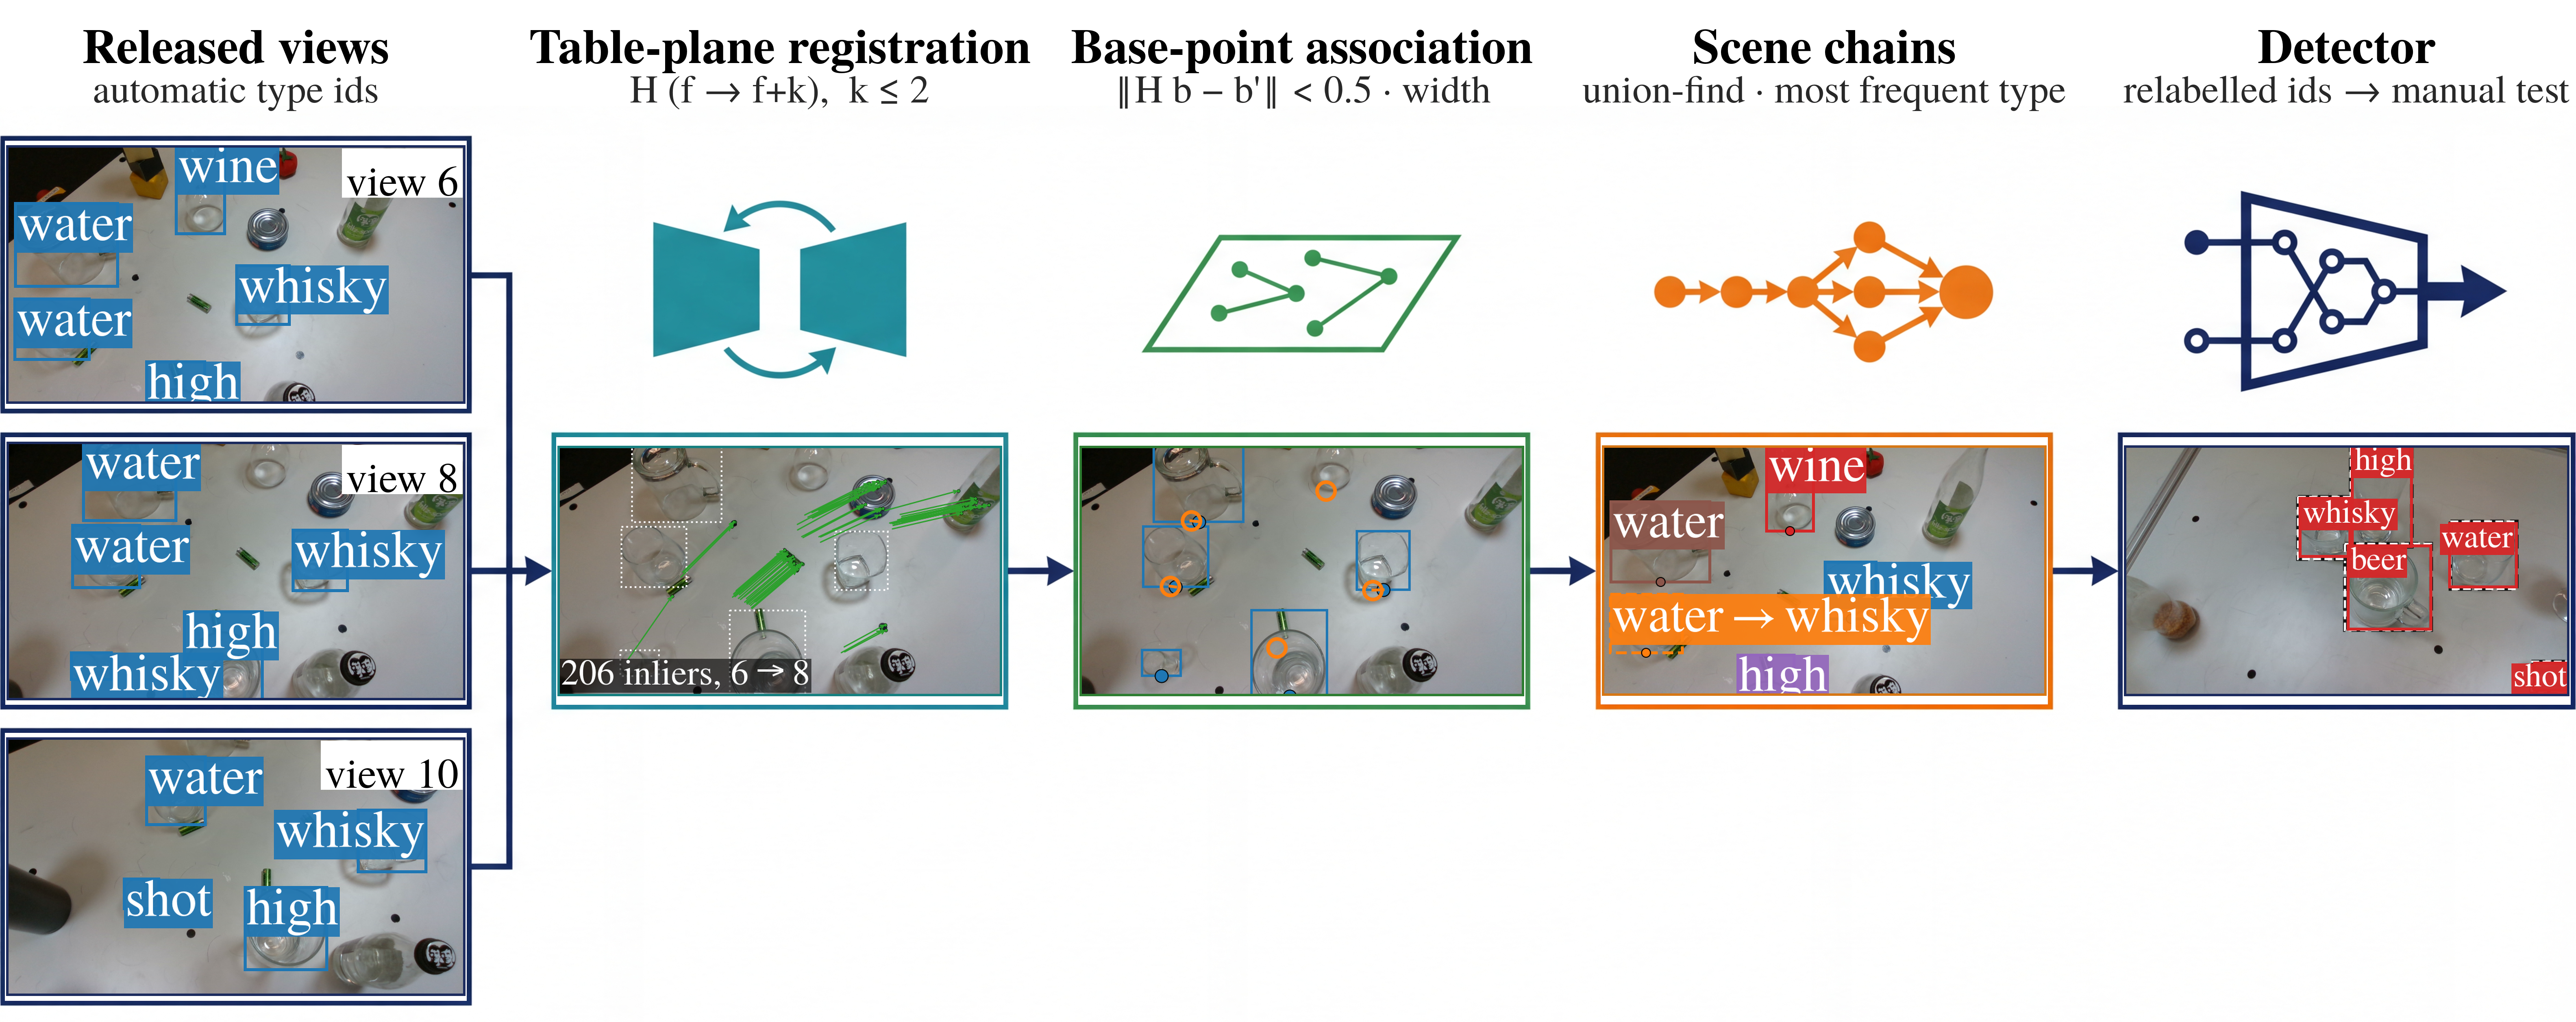
\includegraphics[width=\textwidth]{figures/figure_overview.png}
\caption{Overview. Views of a static scene are registered through the table plane by background features; each box is carried by its base point, which lies on that plane, and linked to the box it lands on; union-find merges the links into one chain per glass, whose most frequent type replaces every type id in it; the relabelled set trains a detector scored on the hand-labelled splits. Photographs: views 6, 8 and 10 of one training scene with released boxes and types; inliers of the view 6 to 8 homography as displacement vectors; base points of view 6 carried into view 8 (open) and linked to those of view 8 (filled); view 6 with one colour per chain and a dashed box where the vote replaced the type; a scene-vote detector's boxes with confidences on a manual OOD test frame, manual boxes dashed; frame chosen where every manual box is detected with the correct type and nothing else. Photographs and overlays are real; the stage symbols are schematic.}
\label{fig:flow}
\end{figure*}

\section{Proposed method}
\label{sec:method}
\subsection{Type labels disagree on the same object}
\label{sec:noise}
GlassNICOL assigns type automatically (we call this step the labeller): the height of a depth cluster above the table plane, measured in the capped pass, is matched to the nearest of six known glass heights (5, 9, 11, 13, 17.5 and 22\,cm) within 3\,cm~\cite{gajdosech2025glassnicol}. Height is measured per view, but type is constant for the object, so one glass should carry one type across the 25 views of its scene. We take the \AdjFramePairs{} consecutive frame pairs of the training scenes, register frame $f$ to $f{+}1$ by background features, carry each box through the registration and match it to the box it overlaps in $f{+}1$ at intersection over union (IoU) above $0.5$; pairs whose registration fails are matched unwarped. Of the \FlipPairsReg{} matched pairs, \FlipCountReg{} (\FlipRateReg\%) carry a different type (Fig.~\ref{fig:noise}), \FlipNeighbourPct\% of them between glasses of neighbouring height.

The hand-labelled official splits pass the same registered test: \ManStdFlips{} flips in \ManStdPairs{} matched pairs on the standard test, at most \ManOODFlips{} in \ManOODPairs{} (\ManOODFlipRate\%) on the out-of-distribution (OOD) test. The inconsistency is the labeller's, not the scenes'. The same labeller also places two boxes on one glass (IoU above 0.5) in \DupFrames{} of 2,375 training frames (\DupDiffType{} of \DupPairs{} such pairs with different types); the manual splits contain none.

\begin{figure}[t]
  \centering
  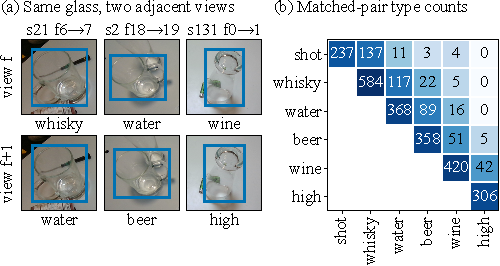
\includegraphics[width=\columnwidth]{figures/figure_labelnoise.pdf}
  \caption{Automatic type labels are not constant on one object. (a) The same glass in adjacent training views $f$ and $f{+}1$, cropped from released frames with the released box and type. (b) Released types of the \FlipPairsReg{} box pairs matched across adjacent views after background registration, each unordered pair counted once; \FlipCountReg{} (\FlipRateReg\%) disagree, \FlipNeighbourPct\% of them between neighbouring heights. Manual test labels flip \ManStdFlips/\ManStdPairs{} and \ManOODFlips/\ManOODPairs.}
  \label{fig:noise}
\end{figure}

The misreads mostly join neighbouring heights and mostly run downward. Treating the views of one glass on an adjacent-frame chain (the tracklets of Section~\ref{sec:vote}) as repeated readings and estimating the labeller's confusion by expectation--maximisation~\cite{dawid1979em}, a water glass is read as a shorter type in \EmDownWater\% of views and as a taller one in \EmUpWater\%, a beer glass \EmDownBeer\% against \EmUpBeer\%, a wine glass \EmDownWine\% against \EmUpWine\%, a highball \EmDownHigh\%; only the shot glass, which has no shorter type, is misread upward, as whisky in \EmUpShot\% (Table~\ref{tab:conf}). Class shares also differ between the training scenes and the six test scenes: the shot:whisky ratio is \RatioRawTrain{} in training, \RatioManualStd{} on the standard test and \RatioManualOOD{} on the OOD test. The release does not say whether that is the labeller's or the staging's; a vote over views leaves it unchanged either way.

\begin{table}[t]
\centering
\caption{The labeller's confusion, estimated from adjacent-frame view chains by expectation--maximisation: percentage of views in which a glass of the true type (column) is read as each type (row). Misreads of every type but the shortest go toward shorter glasses.}
\label{tab:conf}
\setlength{\tabcolsep}{4pt}
\renewcommand{\arraystretch}{1.0}

\begin{tabular}{lrrrrrr}
\toprule
Read as & shot & whisky & water & beer & wine & high \\
\midrule
\inputrows{conf_v11_rows.tex}\bottomrule
\end{tabular}
\end{table}

\subsection{Association through the table plane}
\label{sec:assoc}
Frames $f$ and $f{+}k$ of a scene, $k\le\SceneHops$, are registered by background features: up to 1,500 ORB (oriented FAST and rotated BRIEF) features~\cite{rublee2011orb} are extracted outside the label boxes, which are dilated $1.2\times$ and masked out, matched under a $0.75$ ratio test, and a homography is fitted by RANSAC (random sample consensus)~\cite{fischler1981ransac} at a 3-pixel threshold and kept when at least 30 matches and half of them are inliers. The background is the table, so the homography is the table plane's and carries a glass's base point, the bottom-centre of its box, exactly; the rest of the box moves with parallax. Each box of $f$ is carried into $f{+}k$ by its base point and linked, one-to-one in order of distance, to the box whose base point lies within \SceneTol{} of the mean box width. Union-find merges links across the scene into chains, one glass seen in several views, under one constraint: a chain holds at most one box per frame, and a link that would violate it is refused (\SceneRefused{} of the links proposed by the \SceneRegPairs{} registered pairs).


\begin{table}[t]
\centering
\caption{Association ablation on the training split: the first row is the earlier partial-affine, adjacent-frame baseline; the other rows use the homography registration and vary the linking cue (warped-box overlap or base point) and the hop count. Chains; median votes per box; boxes with three or more votes (\%); type ids changed (\%); manual-split checks (first row: flips among matched adjacent-view pairs, Section~\ref{sec:noise}; other rows: disagreeing boxes).}
\label{tab:assoc}
\setlength{\tabcolsep}{2.5pt}
\renewcommand{\arraystretch}{1.0}

\begin{tabular}{lrrrrrr}
\toprule
Association & Chains & Votes & $\geq$3 & Chg. & Std. & OOD \\
\midrule
\inputrows{assoc_v14_rows.tex}\bottomrule
\end{tabular}
\end{table}

\subsection{Vote, coverage and validity}
\label{sec:vote}
Each chain takes its most frequent type (a plurality); ties are left unchanged. Only the type id changes: no box moves, no image is added or removed, and roster and hyperparameters are identical to the raw arm. The association runs on all 95 training scenes (the detector roster below uses 70 of them, on which 11.7\% of type ids change): \SceneRegPairs{} of \SceneTriedPairs{} frame pairs register; \ChainBoxes{} boxes fall into \SceneChains{} chains with a median of \SceneMedianLen{} views per box, \SceneBoxesGeThree{} boxes (\SceneBoxesGeThreePct\%) are voted on by three views or more, \SceneChanged{} boxes (\SceneChangedPct\%) change type and \SceneTied{} in tied chains keep their label. Table~\ref{tab:assoc} separates the ingredients: the adjacent-frame overlap vote of our earlier baseline, which registered \ChainFramePairsReg{} of \AdjFramePairs{} pairs by a partial-affine warp, gives \TrkChains{} chains, \TrkSingletons{} of them a single box, a median of \TrkMedianVotes{} votes per box, and changes \TrkChanged{} boxes (\TrkChangedPct\%). Under the homography registration, overlap linking over one hop already lengthens the chains; the base point and the second hop each add votes, and only their combination gives the most votes with no merged glasses of different type on either manual split. That baseline is the tracklet arm of Section~\ref{sec:results}. The validation split is left as released: checkpoint selection uses generic average precision (AP), so type ids never enter it.

\noindent\textbf{Validity.} Manual types are constant per object, so on the hand-labelled splits every within-chain type disagreement is a merged pair of glasses. The association above produces \ManualChainStd{} disagreeing boxes on the standard split and \ManualChainOOD{} on the OOD split, with median chain lengths of \ManualMedianStd{} and \ManualMedianOOD{} (\ManualGeThreeStd{} and \ManualGeThreeOOD{} boxes in chains of three or more). The hop count and tolerance were chosen by this check on a grid of two to four hops and three tolerances before any scene-vote detector was trained, so the zero above is an in-sample value: at the chosen tolerance, three and four hops leave four disagreements on the standard split and two hops none; a one-hop run made afterwards leaves two on the OOD split. The manual splits never enter training.

\noindent\textbf{Scope.} A vote over views removes disagreement that varies by view and inherits whatever is constant across views, such as the shot/whisky share difference above; Section~\ref{sec:pairs} scores each pair.

\section{Experimental results}
\label{sec:results}
\subsection{Setup}
\label{sec:setup}
\noindent\textbf{Data.} The official GlassNICOL head-camera split~\cite{gajdosech2025glassnicol}: 2,375 training images from 95 scenes, 125 validation images, and hand-labelled standard and OOD tests (66 and 75 images, 3 scenes each). The training roster, fixed before this experiment, uses \ScenesTrain{} of the 95 scenes (\ImagesTrainScene{} images).

\noindent\textbf{Detector and regime.} YOLO11n~\cite{jocher2024yolo11} (2.59M parameters~\cite{sapkota2025yolo}), $640\!\times\!640$ inputs, batch 64, AdamW~\cite{loshchilov2019adamw} at $\mathrm{lr}_0=10^{-3}$, cosine decay over \SceneEpochs{} epochs. All arms train under the same repeated-exposure regime: the \SceneRepeatSlots{} training images whose transparent and chalk-coated captures register by the same background matching appear twice, \SceneSlots{} slots and \SceneUpdates{} optimiser updates, and the arms differ only in training type ids: raw, tracklet vote, scene vote. Seeds 1337, 3407 and 4567 run on accelerator A (an H200 GPU) and seeds 1337 and 5678 on accelerator B (an RTX PRO 6000 GPU); a cell is one (accelerator, seed) set of the three arms, an arm being one label variant on the shared roster.

\noindent\textbf{Scoring.} The checkpoint with the best validation generic AP is scored at confidence floor $0.001$ with non-maximum suppression (NMS) at IoU $0.7$: COCO (Common Objects in Context) box AP over IoU $0.50$--$0.95$~\cite{lin2014coco}; generic AP collapses the six types to one. Released annotation ids start at zero and are renumbered from one for pycocotools. Type accuracy is the fraction of ground-truth boxes localised by the compared arms (IoU $\geq0.5$, confidence $\geq0.25$) with the correct type; recall is the localised fraction per arm.

\noindent\textbf{Protocol.} The comparison was preregistered before any scene-vote detector was trained: the three arms, the five cells, the checkpoint rule, the four metrics above, and four predictions, a positive mean type-accuracy gain over the raw labels on both splits (P1), an OOD gain exceeding the tracklet vote's (P2), recall and generic AP within two points (P3), and a positive OOD gain in at least four of five cells (P4). The sealed protocol, every evaluation receipt and the code are at \url{https://github.com/HeunSeungLim/glassnicol-scene-relabel}. Every contrast is read as a mean over cells with the count of positive cells beside it~\cite{bouthillier2021variance}.

\begin{table*}[t]
\centering
\caption{Raw, tracklet-vote and scene-vote training labels on the official test splits (manual labels), mean $\pm$ standard deviation over seeds per accelerator A or B (number of seeds in parentheses; with two seeds the deviation has one degree of freedom). Six: six-class AP; Gen: generic AP; Rec: localisation recall; Type: type accuracy on boxes localised by all three arms, a different box set from the pairwise contrasts of Table~\ref{tab:cells}; all in percent.}
\label{tab:arms}
\setlength{\tabcolsep}{4pt}
\renewcommand{\arraystretch}{1.0}

\begin{tabular}{llrrrrrrrr}
\toprule
& & \multicolumn{4}{c}{Standard} & \multicolumn{4}{c}{OOD} \\
\cmidrule(lr){3-6}\cmidrule(lr){7-10}
Accel. (seeds) & Labels & Six & Gen & Rec & Type & Six & Gen & Rec & Type \\
\midrule
\multirow{3}{*}{H200 (3)} & raw & 68.9$\pm$3.9 & 84.0$\pm$2.2 & 89.6$\pm$1.2 & 86.1$\pm$4.2 & 53.8$\pm$7.1 & 66.1$\pm$0.9 & 77.9$\pm$4.1 & 79.9$\pm$7.3 \\
& tracklet vote & 64.6$\pm$4.6 & 84.8$\pm$3.0 & 88.6$\pm$1.2 & 86.3$\pm$3.0 & 54.0$\pm$4.6 & 67.3$\pm$1.0 & 81.0$\pm$0.8 & 82.6$\pm$2.3 \\
& scene vote & 61.9$\pm$2.7 & 81.6$\pm$3.5 & 87.6$\pm$1.2 & 82.6$\pm$2.0 & 60.2$\pm$3.2 & 65.9$\pm$1.4 & 77.1$\pm$4.1 & 83.8$\pm$9.4 \\
\midrule
\multirow{3}{*}{RTX (2)} & raw & 60.1$\pm$1.6 & 84.4$\pm$2.2 & 92.5$\pm$1.3 & 77.5$\pm$2.8 & 53.5$\pm$0.4 & 67.4$\pm$1.5 & 82.3$\pm$2.0 & 68.6$\pm$5.6 \\
& tracklet vote & 67.0$\pm$2.8 & 87.2$\pm$0.7 & 89.5$\pm$3.8 & 83.9$\pm$0.7 & 54.8$\pm$7.4 & 66.9$\pm$2.9 & 78.8$\pm$1.4 & 76.4$\pm$7.9 \\
& scene vote & 65.9$\pm$2.6 & 83.8$\pm$2.5 & 90.4$\pm$3.4 & 84.3$\pm$5.2 & 61.5$\pm$1.5 & 66.8$\pm$2.3 & 80.3$\pm$1.6 & 84.9$\pm$0.1 \\

\end{tabular}
\end{table*}

\begin{table}[t]
\centering
\caption{Type-accuracy gain of the scene vote in every (accelerator, seed) cell, in points on the manual boxes both compared arms localise: over the raw labels; 95\% paired frame-bootstrap interval (2,000 draws).}
\label{tab:cells}
\setlength{\tabcolsep}{3pt}
\renewcommand{\arraystretch}{1.0}

\begin{tabular}{llrlrl}
\toprule
& & \multicolumn{2}{c}{Standard} & \multicolumn{2}{c}{OOD} \\
\cmidrule(lr){3-4}\cmidrule(lr){5-6}
Accel. & Seed & Gain & 95\% interval & Gain & 95\% interval \\
\midrule
\inputrows{cells_v14b_rows.tex}\bottomrule
\end{tabular}
\end{table}

\begin{table}[t]
\centering
\caption{Type-accuracy change of the scene vote over the raw labels on the manual test boxes of each confusable pair (localised by both arms): mean over the \SvCells{} cells and the number of positive cells.}
\label{tab:pairs}
\setlength{\tabcolsep}{5pt}
\renewcommand{\arraystretch}{1.0}

\begin{tabular}{lrrrr}
\toprule
& \multicolumn{2}{c}{Standard} & \multicolumn{2}{c}{OOD} \\
\cmidrule(lr){2-3}\cmidrule(lr){4-5}
Pair & Mean & Positive & Mean & Positive \\
\midrule
\inputrows{pairs_v13_rows.tex}\bottomrule
\end{tabular}
\end{table}

\subsection{What the labels change}
Table~\ref{tab:arms} pools the seeds per accelerator and Table~\ref{tab:cells} lists every cell. Two contrasts hold across cells. Out of distribution, six-class AP rises by \SvSixOODVsRawGain{} points over the raw labels in \SvSixOODVsRawPos{} of \SvCells{} cells (across-cell 95\% $t$-interval \SvSixOODVsRawCI) and by \SvSixOODVsTrkGain{} over the tracklet vote (\SvSixOODVsTrkCI), which the tracklet vote itself did not move (\SvSixOODTrkVsRawGain). On the standard split localisation recall falls by 2.0 points, in every cell (\SvRecStdVsRawCI). The type-accuracy gains are larger but less certain: out of distribution the scene vote gains \SvTypeOODVsRawGain{} points over the raw labels, positive in \SvTypeOODVsRawPos{} of \SvCells{} cells, with per-cell frame-bootstrap intervals above zero in \SvOODAbove{} cells, reaching it in \SvOODStraddle{} and below it in \SvOODBelow{} (Table~\ref{tab:cells}) and an across-cell interval of \SvTypeOODVsRawCI{} (cell standard deviation \SvTypeOODVsRawSD); over the tracklet vote it gains \SvTypeOODVsTrkGain{} (\SvTypeOODVsTrkPos{} of \SvCells). On the standard split type accuracy changes by \SvTypeStdVsRawGain{} over the raw labels and \SvTypeStdVsTrkGain{} over the tracklet vote, with \SvStdAbove{} cell above zero and \SvStdBelow{} below, and six-class and generic AP change by \SvSixStdVsRawGain{} and \SvGenStdVsRawGain. The one cell that loses on both splits, seed 4567 on A, does so by eight and ten points; every other cell gains out of distribution by six points or more.

\noindent\textbf{Preregistered predictions.} P1 held: the mean type-accuracy gain over the raw labels is positive on both splits, \SvTypeStdVsRawGain{} and \SvTypeOODVsRawGain. P2 held: out of distribution the scene vote's gain exceeds the tracklet vote's gain of \SvTypeOODTrkVsRawGain. P4 held: \SvTypeOODVsRawPos{} of \SvCells{} OOD cells are positive. P3 did not hold: on the standard split localisation recall falls by 2.0 points, just past the two-point bound, and generic AP by 1.7; out of distribution both stay within it. Scoring the last epoch instead (post hoc, rows released with the code) gives, over the raw labels, type accuracy \SvLTypeStdVsRawGainL{} on the standard split (\SvLTypeStdVsRawPosL{} of \SvLCells{} cells, so P1 holds only under the preregistered rule) and \SvLTypeOODVsRawGainL{} out of distribution (\SvLTypeOODVsRawPosL{} of \SvLCells), six-class AP \SvLSixStdVsRawGainL{} and \SvLSixOODVsRawGainL, recall \SvLRecStdVsRawGainL{} and \SvLRecOODVsRawGainL{} (\SvLRecStdVsRawPosL{} and \SvLRecOODVsRawPosL{} of \SvLCells{} cells positive). The OOD gain holds under both rules; the standard-split recall loss does not.

\subsection{Where the vote helps and where it cannot}
\label{sec:pairs}
Table~\ref{tab:pairs} scores each confusable pair against the raw labels. Out of distribution every pair gains on average: whisky/water \PairSWhiskyOODMean{} points (\PairSWhiskyOODPos{} cells), wine/high \PairSWineOODMean{} (\PairSWineOODPos), water/beer \PairSWaterOODMean{} (\PairSWaterOODPos) and shot/whisky \PairSShotOODMean{} on average (\PairSShotOODPos), a mean carried by one cell at \PairSShotOODMax{} with a median of \PairSShotOODMedian; that is the pair whose share differs most between training and test and which the tracklet vote could not move. On the standard split the two shortest pairs lose, shot/whisky \PairSShotStdMean{} and whisky/water \PairSWhiskyStdMean, while water/beer and wine/high gain \PairSWaterStdMean{} and \PairSWineStdMean; the earlier tracklet-vote protocol's refutation condition on confusable-pair agreement is met there.

\section{Discussion and limitations}
\label{sec:limits}
The vote cannot change class shares. Whisky is \WhiskyShareRaw\% of raw training boxes, \WhiskyShareStd\% of the standard test and \WhiskyShareOOD\% of the OOD test, and the shot:whisky ratio is \RatioRawTrain{} in raw training labels, \RatioSceneTrain{} after the scene vote, against \RatioManualStd{} and \RatioManualOOD{} in the tests. Decoding the chains under the confusion of Table~\ref{tab:conf} instead of by the most frequent type moves the ratio no closer; deciding whether the difference is the labeller's or the staging's needs the per-box height the labeller measured, which is not released; we did not recompute it from the released depth, nor run a pose-based reprojection baseline.

The association is only as good as the table: frames without enough background features stay unlinked, a chain cannot vote on a glass the labeller never boxed, and the \DupFrames{} frames with two boxes on one glass are voted on as two objects.

The gain is out of distribution. On the standard split the scene vote changes type accuracy by \SvTypeStdVsRawGain{} points, does not beat the tracklet vote, and costs 2.0 points of recall and 1.7 of generic AP under the preregistered checkpoint rule; one seed on A loses on both splits, and with five cells the OOD type-accuracy mean sits inside the seed spread; the six-class AP contrast and the per-cell intervals carry the claim. The official test splits have three scenes each, and the tracklet contrast re-run for seed 1337 on accelerator B moved by \XHostTypeStd{} and \XHostTypeOOD{} type-accuracy points, so single cells are read against that swing. Checkpoint selection by validation generic AP ($r^2=\SelRsq$ with test six-class AP) is the same for every arm, so the arms differ only in their labels.

\section{Conclusion}
GlassNICOL's automatic type ids disagree on the same glass in \FlipRateReg\% of adjacent-view pairs; its hand labels do not. The table plane links the views of a glass, and a vote over them gives one type per object: \SceneChangedPct\% of type ids change and no box moves. Detectors trained on the corrected labels gain out of distribution: six-class AP by \SvSixOODVsRawGain{} points over the raw labels in every cell and \SvSixOODVsTrkGain{} over an adjacent-frame vote, type accuracy by \SvTypeOODVsRawGain{} and \SvTypeOODVsTrkGain{} in four of five cells, with across-cell intervals that include zero. On the standard split they gain nothing and lose two points of recall.

\clearpage
\bibliographystyle{IEEEbib}
\bibliography{references}
\end{document}
